\section{Unit Experiments}
\label{text:experiments/unit}

\subsection{Horizon Weighting for Goal Objective Function}
In Table \ref{table:goal_horizon_weighting}, the convergence speed of both the "unweighted" \ref{eq:goal_unweighted} and the "weighted" \ref{eq:goal_weighted} objective formulation are compared over 100 runs in a simplified setup, with no pedestrian in the scene and random assignments of the robot's initial and goat state. Weighting the cost terms non-uniformly over the horizon enables finding "trade-offs" of a locally higher cost for faster global convergence, such as gaining speed in a non-goal-direction at the beginning of the horizon but leads to a smaller cost at the end of it.

\begin{table}[!ht]
\begin{center}
\begin{tabular}{c|c|c}
\bf Goal Objective & \bf MSI & \bf M95OD \\
\hline
Weighted & 9.58 & 5.86 \\
\hline
Un-Weighted & 9.64 & 6.64 \\
\end{tabular}
\caption{Comparison of key performance parameter of the optimization using either the "un-weighted" (Equation \ref{eq:goal_unweighted}) or the "weighted" (Equation  \ref{eq:goal_weighted}) goal objective formulation over 100 runs in a simplified environment setup. For further details please have a look into the example notebook: \href{https://github.com/simon-schaefer/mantrap/blob/master/examples/module_goal.ipynb}{examples/module\_goal}.}
\label{table:goal_horizon_weighting}
\end{center}
\end{table}

\subsection{Alternatives to Interactive Objective Function}
Next to the interactive objective function $J_{int}(\cdot)$, described in Section \ref{text:approach/objective/interactive}, there are several other ways to formulate it. Instead of taking the full trajectory distribution into account for computing the distance measure between the unconditioned $\distwo[]$ and the conditioned trajectory distribution $\dist[]$, it can be approximated by computing the expected value over sample pairs. Consequently, the distance measure breaks down to a weighted sum over $L_2$-norms for each discrete time-step within the time horizon and for every trajectory pair, which are efficient to compute.

\begin{equation}
D_{int}^{sp} = \sum_{samples} \sum_T ||\xpedwo[s]_t - \xped[s]_t||_2
\end{equation}

The samples are deterministic trajectories and can be numerically differentiated efficiently, using central difference expressions. As previously described, it might be more meaningful to compare velocity or acceleration instead of positions.

\begin{align}
J_{int, sa}^{k} &= \sum_{samples} \sum_T ||\ddxpedwo[s]_t - \ddxped[s]_t||_2	 \\
J_{int, sv}^{k} &= \sum_{samples} \sum_T ||\dxpedwo[s]_t - \dxped[s]_t||_2	 \\
J_{int, sp}^{k} &= \sum_{samples} \sum_T ||\xpedwo[s]_t - \xped[s]_t||_2
\label{eq:interaction_diff}	
\end{align}

Although quite intuitive, it turns out that a sample-wise objective is hard to optimize. This has two predominant reasons: Firstly, it intrinsically relies on a trade-off between computational feasibility (to compute many times per second for an online optimization) and capability to capture the properties of the underlying real distributions sufficiently well. Secondly, when randomly drawn samples are used, stochasticity is introduced into the objective function, which might lead to a different objective value even when evaluated with the same input. When the distribution's means are used instead, the distribution's uncertainty is disregarded.
\newline
In the following, the projection-probability-based interactive loss function in Equation \ref{eq:objective_interact_prob} is compared against the alternative difference-based objectives, presented above in \ref{eq:interaction_diff}. Due to the previously explained limitations instead of sampled trajectories, the mean trajectory is merely being used, thereby neglecting the prediction's variance. For the comparison, a Monte Carlo simulation is used for a set of custom defined scenarios. Due to the uncertainty evolved in the environment dynamics, the performance is evaluated over 10 test runs each. A meaningful comparison should exclude external factors as best as possible, therefore to exclude interactive effects occurring due to other parts of the optimization, other than the compared objective functions, the safety constraint is not used in this experiment. \\ 

\begin{table}[!ht]
\begin{center}
\begin{tabular}{c|c|c|c|c|c|c}
\bf Interactive Objective & \bf MPE & \bf RTD & \bf RCE & \bf ETT & \bf TGD & \bf MSD \\
\hline
diff\_pos & 0.33 & 0.99 & 0.32 & 0.0 & 0.24 & 0.94 \\
\hline
diff\_vel & 0.29 & 0.98 & 0.51 & 0.0 & 0.26 & 1.16 \\
\hline
diff\_acc & 0.21 & 0.98 & 0.55 & 0.0 & 0.27 & 1.24 \\ 
\hline
\rowcolor{baseline_color}
without & 0.31 & 1.0 & 0.27 & 0.0 & 0.23 & 1.08 \\ 
\hline
\rowcolor{our_color}
projection & 0.18 & 0.92 & 0.79 & 0.8 & 0.39 & 1.44 
\end{tabular}
\end{center}
\label{table:interactive_objective}
\end{table}

The experiments show the effect of the interactive objective function: It trades off the required travel time to reach the goal position with increasing the safety and "ease" of the interaction by reducing the pedestrian's efforts and increasing the minimum separation distance. Figure \ref{img:interactive_comp} displays the solution trajectories for an exemplary scenario.  The projection-probability objective accomplishes to increase distance when necessary but gets on track afterward. In opposition, the alternative formulations either fail to establish a sufficient distance to the pedestrian (comp. the second or third image, associated with diff\_pos and diff\_vel) or cannot recover afterward as in the case for the acceleration difference objective.

\begin{figure}[!ht]
\begin{center}
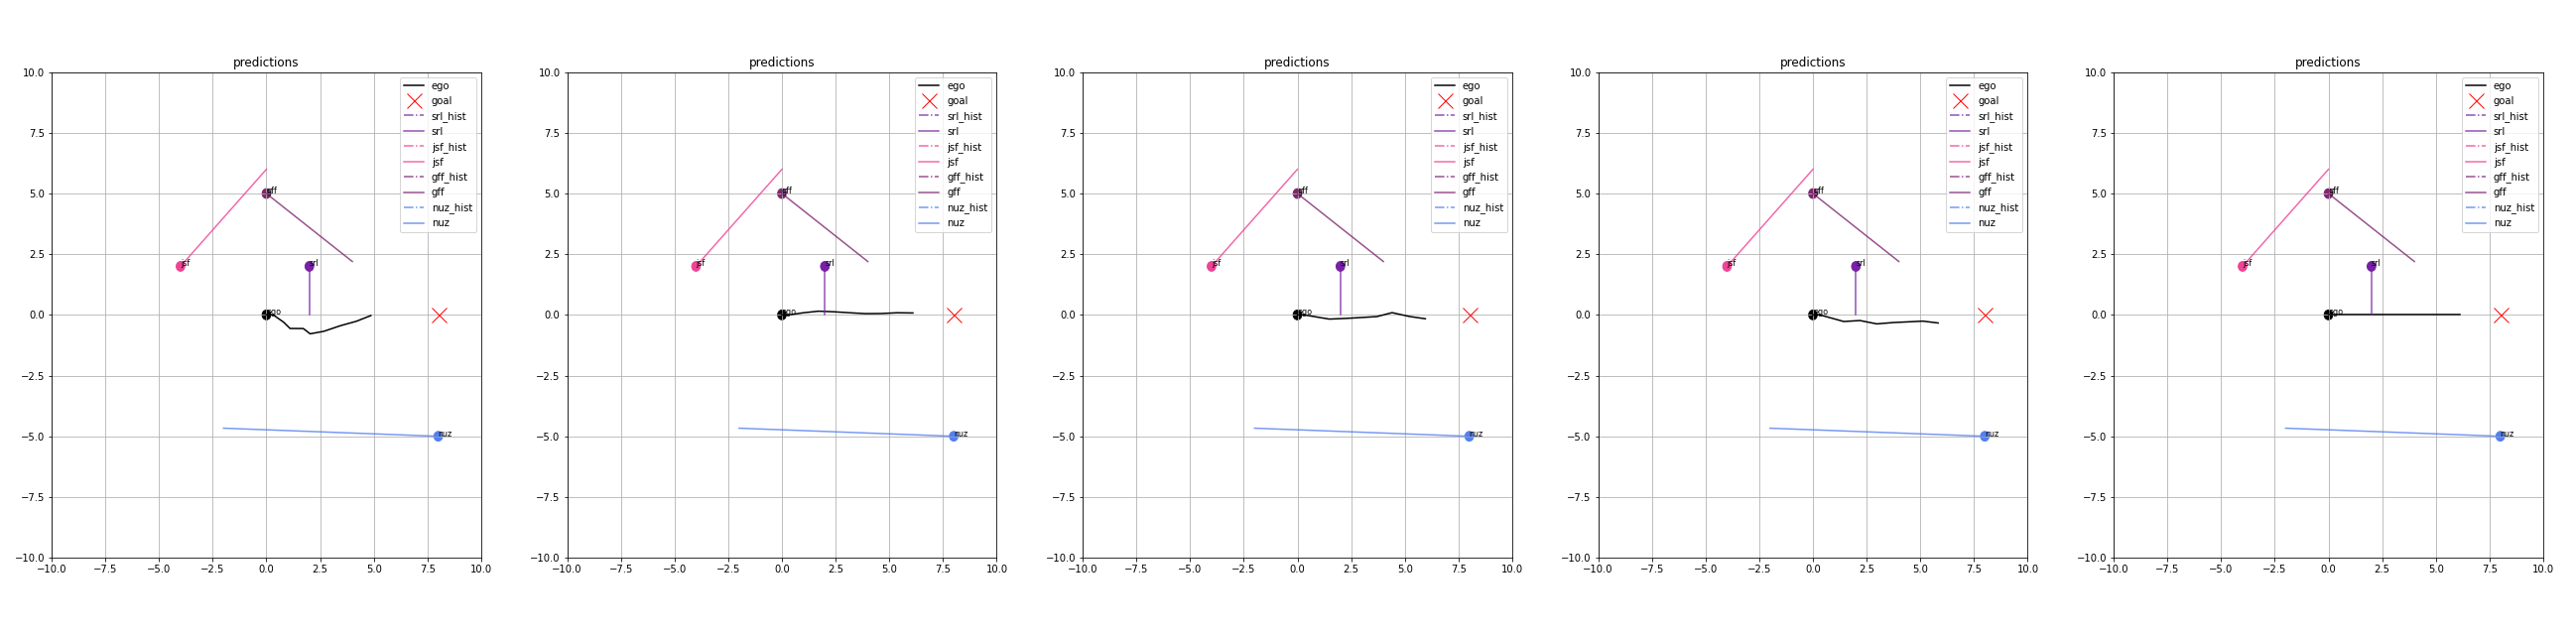
\includegraphics[width=\textwidth]{images/inter_comp_multi.png}
\captionof{figure}{Example solution trajectories for different interactive objective function, beginning from the left: projection, diff\_pos, diff\_vel, diff\_acc, without interactive loss function}
\label{img:interactive_comp}
\end{center}
\end{figure}

\subsection{HJR Value Function Approximation}
The necessity and feasibility of approximating the \ac{HJR} value function have been motivated in Section \ref{text:approach/constraint/safety}. In the following several approximation methods are compared and evaluated.
\newline 
Figure \ref{img:hj_approx_bar} shows the logarithmic approximation error for several pre-computed grid sizes and using linear (as in \cite{Leung2020})) and Nearest Neighbor interpolation methods. LWPR (not shown here) has been tested as well but turned out to be infeasible for a large number of grid points. \footnote{For more information about the implementation of the LWPR value function approximation see \href{https://github.com/simon-schaefer/HJReachibility}{HJ-Reachability Toolbox} on GitHub.} The value function has been computed on a dense grid exactly, and point-wise compared with the grid interpolated approximations for computing the error metric. While linear interpolation widely outperforms Nearest Neighbor, as expected, the absolute error is tiny. As displayed in Figure \ref{img:hj_approx_hist}, the interpolation error is not uniform over all joint state axes, but larger for positional axes (which likely is due to the larger amount of non-linearity in position compared to velocity directions, compare Figure \ref{img:hj_value_function}). Therefore, the number of grid points have not been equally distributed over the axes, but biased to the positional axes (interior), while keeping the overall size of the grid constant.

\begin{figure}[!ht]
\begin{center}
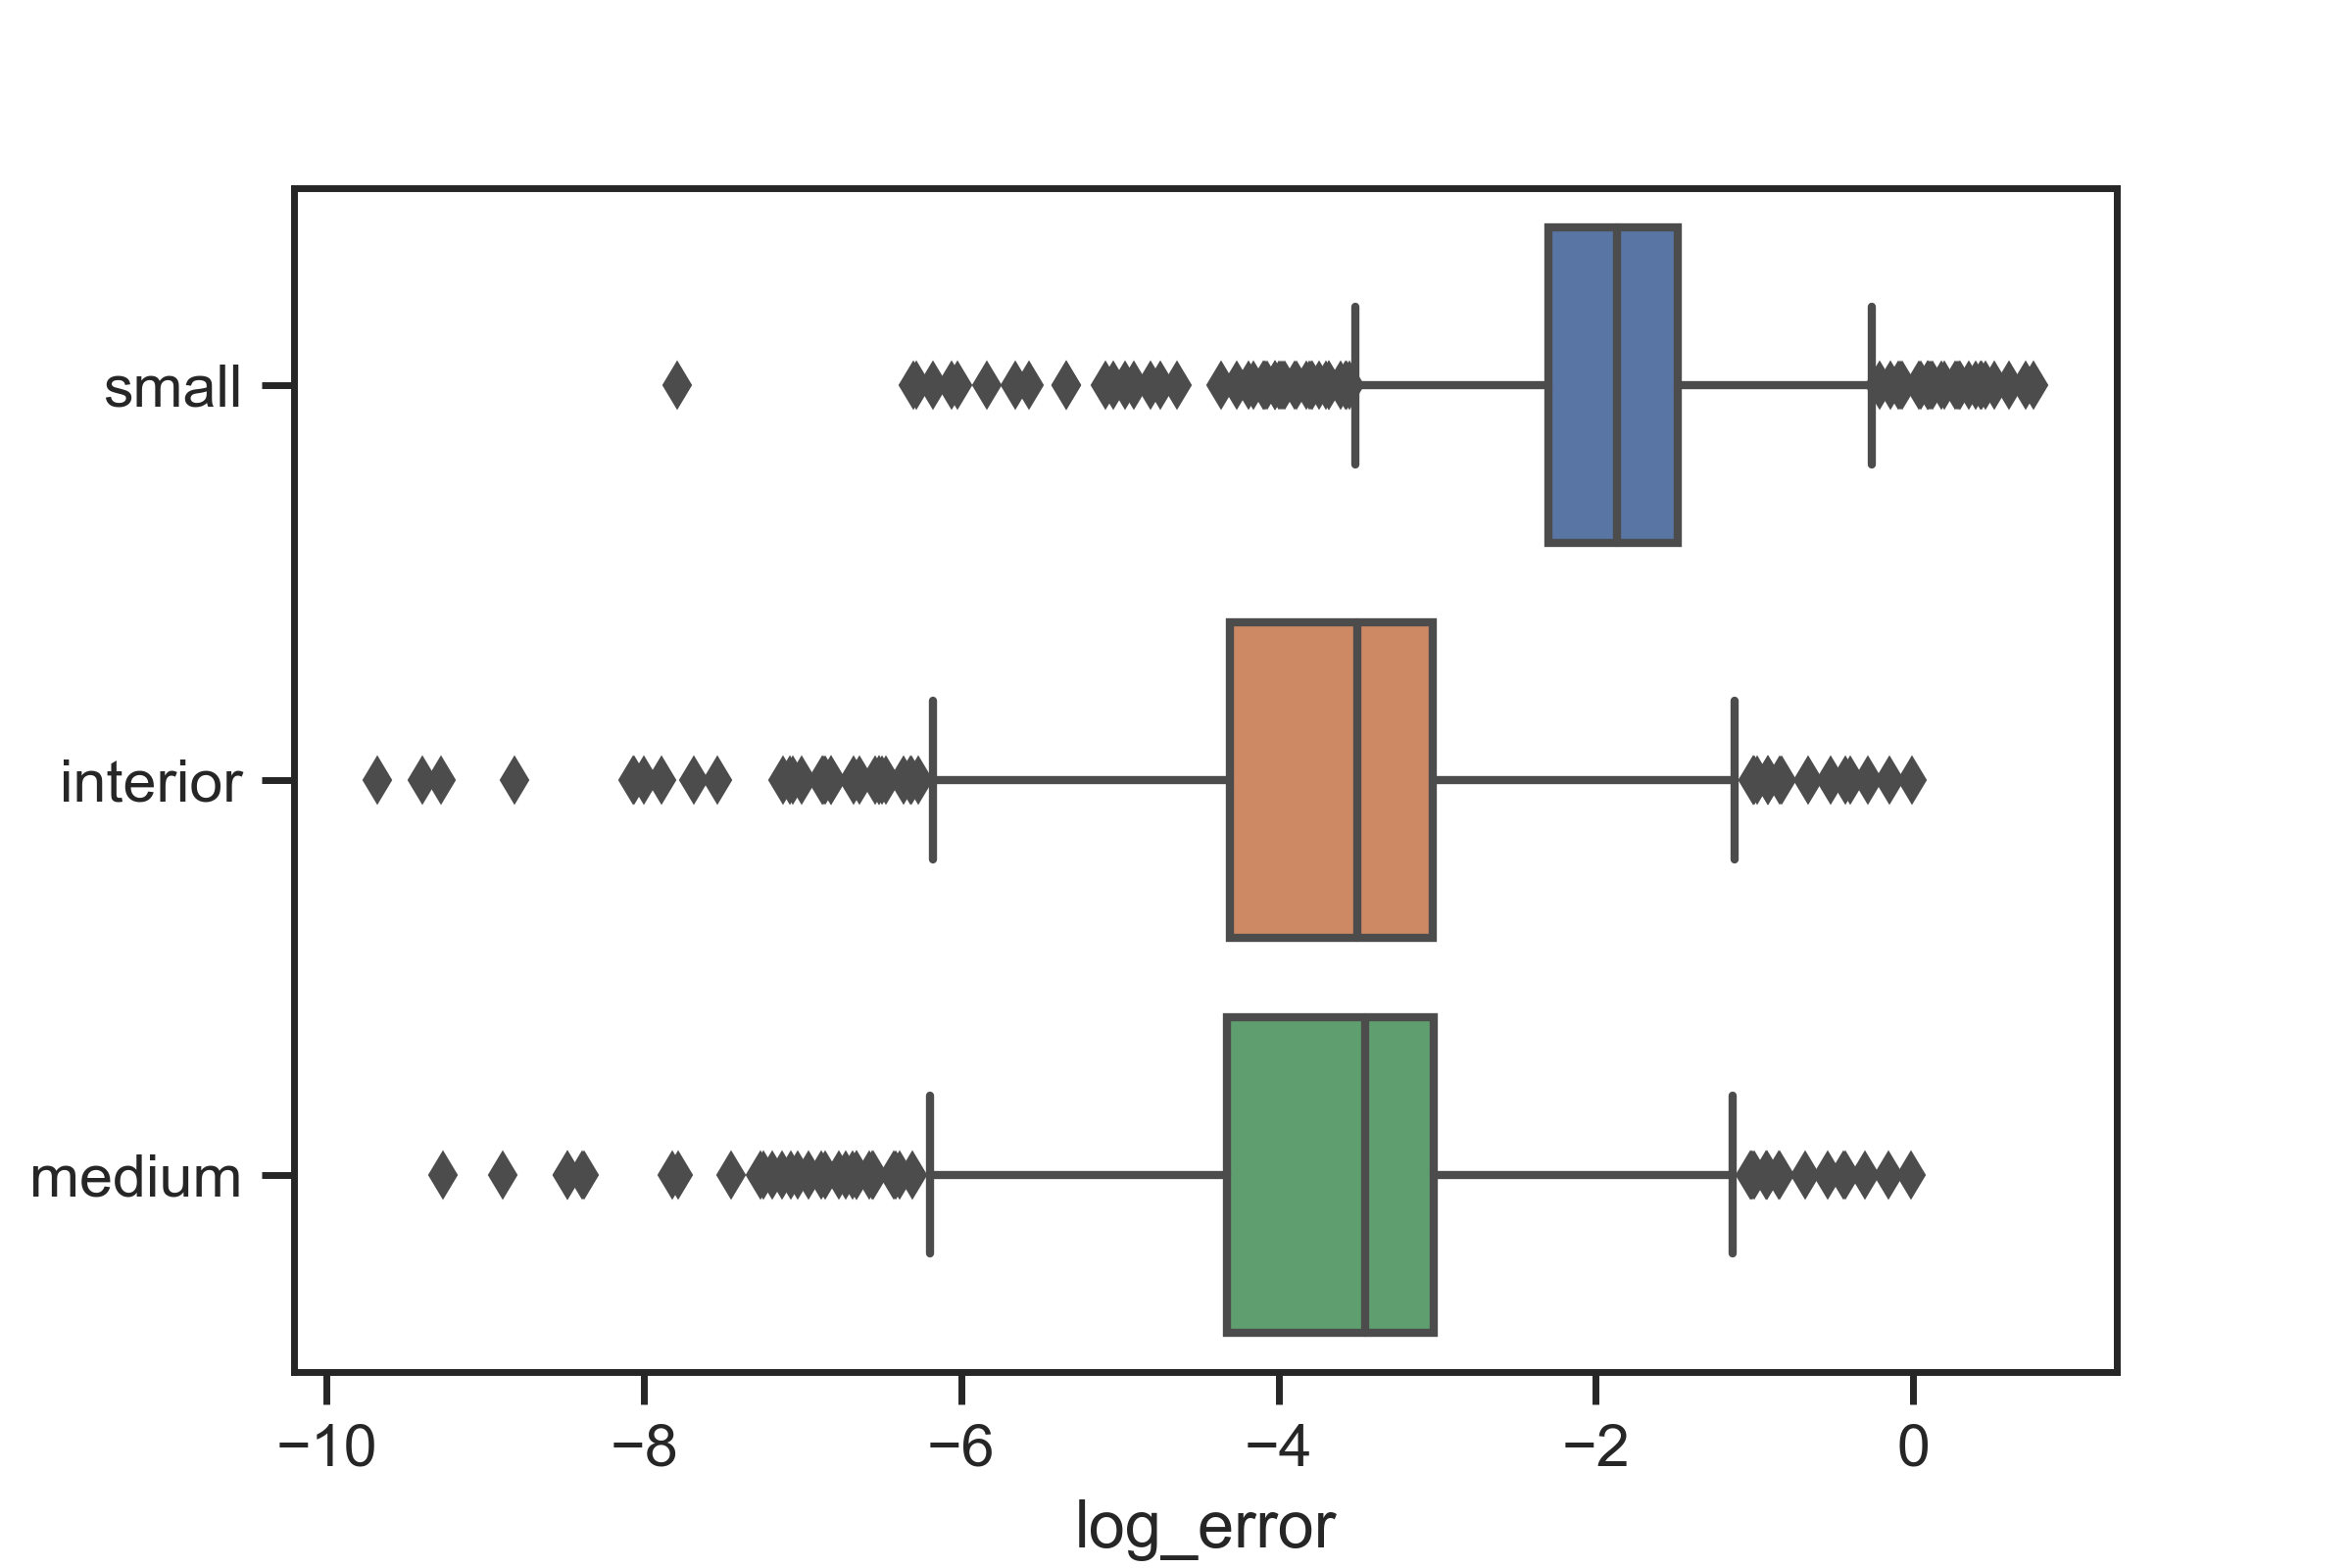
\includegraphics[width=0.45\textwidth]{images/hj_bar_linear.png}
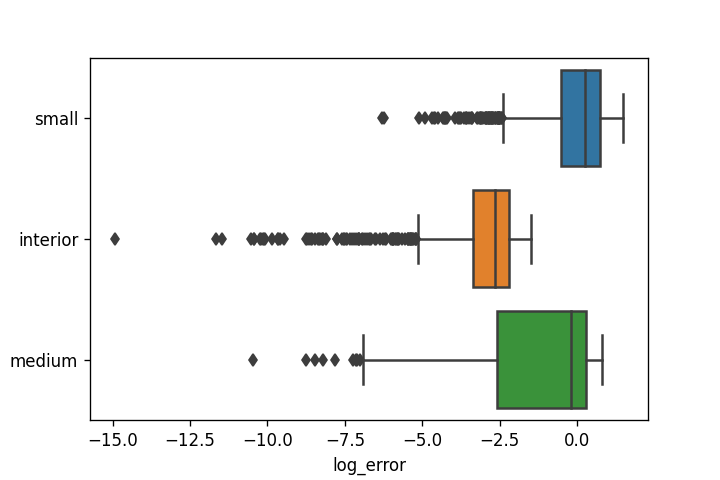
\includegraphics[width=0.45\textwidth]{images/hj_bar_nearest.png}
\caption{Logarithmic value function approximation error using linear (left) and nearest neighbor (right) interpolation methods based on various pre-computed grid sizes (small < interior < medium)}
\label{img:hj_approx_bar}
\end{center}
\end{figure}

\begin{figure}[!ht]
\begin{center}
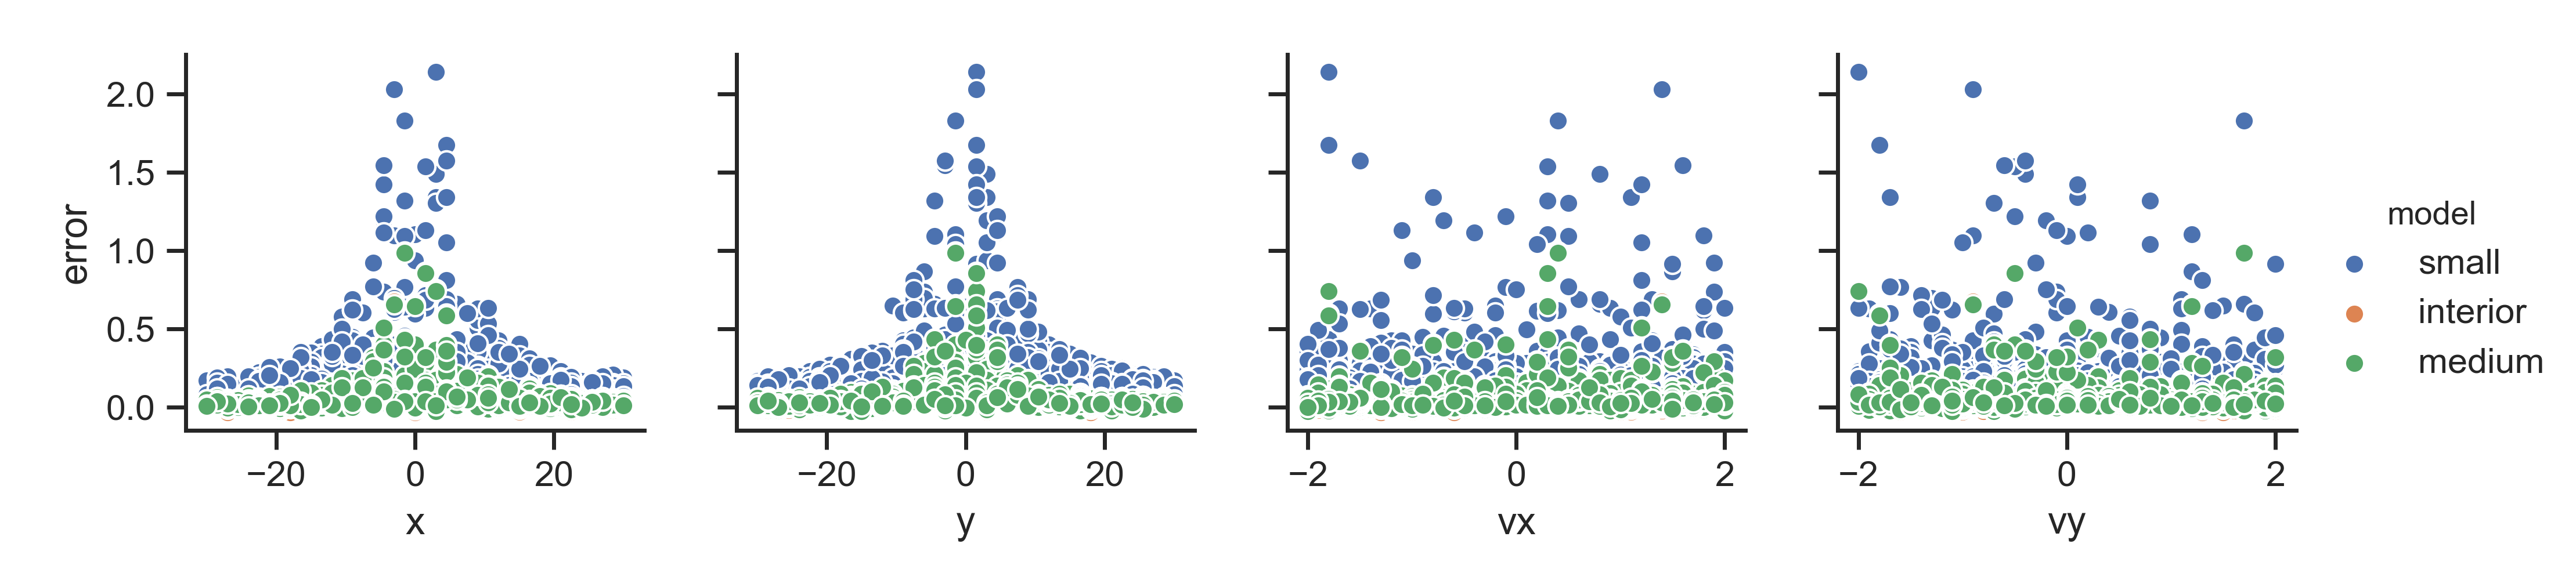
\includegraphics[width=\imgwidth]{images/hj_hist_linear.png}
\caption{Absolute error distribution over joint system state axes using linear interpolation based on various pre-computed grid sizes (small < interior < medium)}
\label{img:hj_approx_hist}
\end{center}
\end{figure}

\subsection{Warm-Starting Methods}
The warm-starting method used in the underlying work simplifies the full trajectory optimization problem to a convex and efficiently computable sub-problem. This process has been described in Section \ref{text:approach/runtime/warm_starting}. This simplified formulation merely takes into account the goal objective as well as a physical constraint imposed by the robot, while neglecting any interaction between robot and pedestrian in the scene. It this way, not only pedestrian-target objectives are ignored, but also constraints enforcing a safe interaction. Despite being efficient to solve, it might return a solution estimate far from the real solution. For example, in the case of a densely crowded area, it might return a solution trajectory, passing very close to other pedestrians, which surely violates the safety constraints of the full formulation. Consequently, the runtime would not be reduced much, if at all. 
\newline
As previously pointed out, there is no simple way of warm-starting interior-point-based methods using preceding solutions. This difficulty motivates finding other warm-starting approaches designed explicitly for crowd-navigation. In the following several other concepts for warm-starting, the underlying optimization problem is introduced and baselined against the used method. The used method, which is solving a simplified, robot-focussed optimization problem, is thereby referred to as \ac{GFW}.

\paragraph{\ac{SCW}} 
SCW follows a similar idea as \ac{GFW}, which is using a simplified formulation of the full optimization problem (Problem \ref{problem:general}) as a wart-start. \ac{GFW}s formulation is thereby extended by the safety constraint $g_{HJR}(\cdot)$ to guarantee that the warm-starting solution is feasible with respect to the system's safety constraint. $g_{HJR}(\cdot)$ is by design independent from pedestrian predictions as well as, for the assumed agent dynamics, widely linear. As a result, \ac{SCW} not only accounts for interactions and feasibility of the warm-started solution trajectory in the full problem but also is comparably efficient to solve.

\paragraph{\ac{PCBW}}
Merkt et alt. \cite{Merkt2018} use nearby pre-computed trajectories to warm-start an optimization problem for controlling a 38-DoF NASA Valkyrie robot in a pick-and-place scenario. Therefore, they encrypt the given initial conditions with problem-specific descriptors, expensively compute solutions for settings distributed over the full state-space, and clusters the pre-computed scenarios using $k$-Means-Clustering. Then, online, the initial conditions are encrypted and efficiently assigned to the closest pre-computed solution with $k$-Nearest-Neighbor classification. 
\newline
For the socially aware trajectory optimization problem in \project, there are several possibilities of encrypting the initial conditions. Finding descriptive but efficient encryption is particularly hard due to the varying number of pedestrians in the scene. To avoid this issue, the internal encoding of a prediction model, such as the latent space $z$ of the Trajectron model \cite{Ivanovic2018}, could be utilized. It is small and constant size makes it very appealing. On the contrary, using a prediction model (latent) encoding would firstly demand the prediction model to have such an encoding (which is only valid (C)\ac{VAE}-based models in the field of pedestrian prediction). Secondly, even if the model does have such an internal encoding, there is no guarantee for it to be meaningful for the task of encrypting a given scene. As not all possible scenes can be pre-solved, it is crucial for the encryption to exhibit a spatial correlation between "close" scenarios, so that matching a non-pre-computed scenario to its closest (spatial) neighbors is feasible. However, the latent space of a prediction model is not guaranteed to have this property. 

\begin{figure}[!ht]
\begin{center}
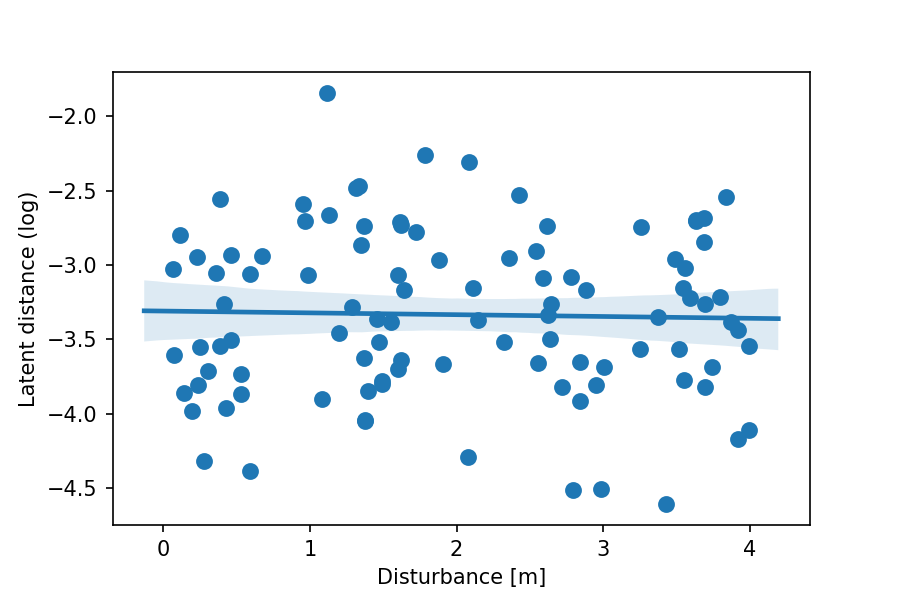
\includegraphics[width=\imgwidth]{images/enc_latent_reg.png}
\caption{Latent space encoding for randomly perturbed scenarios. A multi-pedestrian scenario has been perturbed by randomly shifting the initial positions of randomly picked pedestrian in the scene by the amount displayed on the x-axis, resulting in the logarithmic $L2$-distance mapped on the y-axis. For more information please visit the warm-starting testing notebook \href{https://github.com/simon-schaefer/mantrap/blob/master/examples/warm_start.ipynb}{warm\_start}.}
\label{img:pcbw_encoding_latent}
\end{center}
\end{figure}

Figure \ref{img:pcbw_encoding_latent} illustrates the spatial distribution of the latent space of the Trajectron model. The underlying assumption of a spatial correlation between similar scenarios does not hold. For this reason, a manually-design encoding is used within this work. As previously discussed, designing an encoding for all pedestrian states, the robot and goal state is intrinsically governed by the trade-off between an ample search space and representative capabilities of the encoding. Encryption of the complete environment state increases query time and demands an exponentially larger amount of pre-computed scenarios. As some crowd-navigation works merely take into account the closest or most endangered single pedestrian, a similar idea is considered for encoding. Specifically, the scene descriptors are the local coordinates of the closest pedestrian, with respect to the robot, between it and its goal position. Using a local coordinate frame pointing from the robot's to the goal position saves encoding the goal position as well, by implicitly encoding it. Figure \ref{img:pcbw_encoding_manual} pictures a typical scene encoding. Similarly to \cite{Merkt2018}, the pre-computed solution trajectories are matched to the queried scene using $k$-Nearest-Neighbor classification. 

\begin{figure}[!ht]
\begin{center}
\begin{tikzpicture}

    \node (R) at (0, 0)
    {
\includegraphics[width=.04\textwidth]{images/robot.png}};
    \node (G) at (8, 4)
    {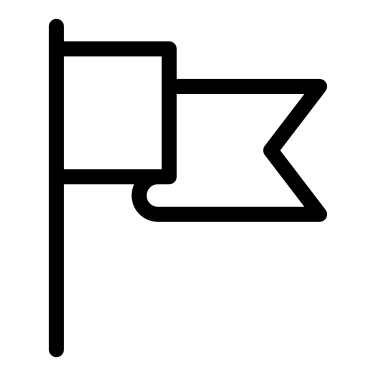
\includegraphics[width=.04\textwidth]{images/flag.png}};
    \node (P1) at (-4, 1)
    {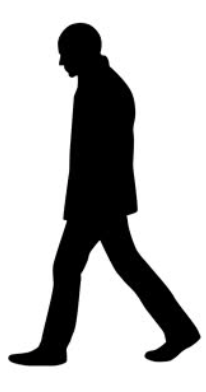
\includegraphics[width=.04\textwidth]{images/walking.png}};
    \node (P2) at (6, 1)
    {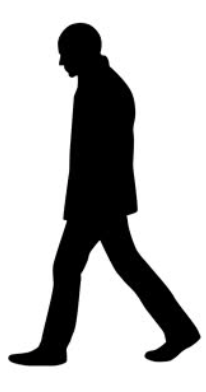
\includegraphics[width=.04\textwidth]{images/walking.png}};
    \node (P3) at (2, 4)
    {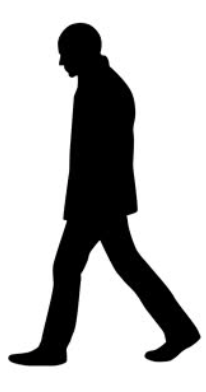
\includegraphics[width=.04\textwidth]{images/walking.png}};

    \draw[->, very thick] (R) to node[midway, sloped, above] {$\eta$} (1, 0.5);
    \draw[->, very thick] (R) to node[midway, sloped, above] {$\mu$} (-0.5, 1);
    \draw[->, dotted] (R) to node[midway, sloped, above] {$(\eta_{P1}, \mu_{P1})$} (P1);
    \draw[->, dotted] (R) to node[midway, sloped, above] {$(\eta_{P2}, \mu_{P2})$} (P2);
   	\draw[->, dotted] (R) to node[midway, sloped, above] {$(\eta_{P3}, \mu_{P3})$} (P3);
   	\draw[->, dotted] (R) to node[midway, sloped, above] {$(\eta_G, 0.0)$} (G);
    
\end{tikzpicture}
\end{center}
\caption{Manual encoding of robot-pedestrian scenario, with local coordinate frame $(\eta, \mu)$ originating in the robots position and pointing in the goal direction.}
\label{img:pcbw_encoding_manual}
\end{figure}

\paragraph{\ac{SPMW}}
It is straightforward to see that the computational complexity of evaluating the interactive terms of the optimization, especially their gradients, is tightly-coupled to the complexity of the underlying prediction model. 
Thus, as an example, it is effortful to compute the gradient of the interactive objective with respect to the robot's trajectory for Trajectron \cite{Ivanovic2018}, but computationally light-weight to do so for the Social Forces environment \cite{Helbing1995}. Following this idea, the \ac{SPMW} method warm-starts the optimization by solving the same (full) optimization problem and using a less complicated environment. The Potential Field prediction model, as described in Section \ref{text:exp_particles}, has been developed for warm-starting. It is worth noting that \ac{SPMW} enables us to improve the efficiency of the optimization and take advantage of prior knowledge. Therefore, the Potential Field model has been designed so that the pedestrian is only affected by the robot when it is close to the pedestrian and in front of it. Consequently, the optimization is driven to a solution in which the robot moves behind or in the distance of each pedestrian.

\paragraph{Evaluation}
Evaluating the performance of the exhibited warm-starting methodologies generally is hard, as for each warm-starting method a set of scenarios can be constructed, in which the resulting warm-started trajectory is very close to the optimal trajectory. As an example \ac{GFW} works well for sparse scenarios, with few pedestrians, while \ac{SCW} performs well, when the robot starts close to a pedestrian. However, in most cases the warm-starting methods decrease the average optimization runtime by $5-10 \%$, while not qualitatively affecting the shape of the solution trajectory. Empirically, \ac{SCW} seems to perform best. Automatically deciding the optimal warm-starting method for a given scenario, as e.g., by leveraging learning-based methods as in \cite{Banerjee2020}, is left for future work.

\subsection{Attention Methods}
Section \ref{text:approach/runtime/filtering} has introduced the concept of attention for filtering the significant pedestrians for evaluating the interactive objective and cutting computational runtime. Next to the purposed euclidean-distance-based attention module, there are several other methodologies for this purpose, out of which two more sophisticated options will be presented in the following:

\paragraph{Forward Reachability Attention}
Forward reachability generally determines the reachable set of an agent given its dynamics and some time-horizon $T_{FR}$. In opposite to back-ward reachability (\ac{HJR}), which has been introduced in Section \ref{text:approach/constraint/safety}, forward reachability merely regards one agent instead of joint systems. Thereby, forward reachability deals with finding the set of all states that the agent can reach from a given set of states $\mathcal{L}$ at time $T_{FR}$. With dynamics $\dot{x} = f(x, u)$, the reachable set $\mathcal{X}_{FR}$ is determined as:

\begin{equation}
\mathcal{X}_{FR} = \{x_T: \in u, \textit{ s.t. } x(\cdot) \textit{ satisfies } \dot{x} = f(x, u), x(0) \in \mathcal{L}; x(T_{FR}) = x_T\}
\end{equation}
 
For single- and double-integrator dynamics, the forward reachable set $\mathcal{X}_{FR}$ turns out to be a circle, due to their isotropy. The radius and center point, thereby, depends on the agent's initial state. Due to the ability to determine these sets analytically, the forward reachability-based attention filter is very computationally efficient to apply.
\newline
Consequently, the forward reachable set attention selects the pedestrian of which the reachable sets overlap with the robot's reachable set for the planning horizon $T_{FR} = T$. If the reachable sets do not overlap, it is not possible for the robot and some pedestrian $k$ to meet within the planning horizon. Then pedestrian $k$ can safely be neglected within the optimization.

\paragraph{Proximate Attention}
The proximate attention module is re-using a concept, that is frequently used in game-theoretic crowd-navigation. Here, the problem is formulated as games between each robot-pedestrian-pair \cite{Bouzat2014}\cite{Nikolaidis2017}. Following this idea, the proximate attention module merely considers the pedestrian, which is closest to the robot (and within a pre-determined euclidean range).

\begin{equation}
\attention_{closest}(\x, \xped[k]) = \left( ||\x - \xped[k]||_2 > D_{Attention} \land \arg \min ||\x - \xped[k]||_2 \right)
\end{equation}

\paragraph{Evaluation}
Table \ref{table:attention} and Figure \ref{img:attention} show the results of a Monte Carlo-based evaluation, averaged over ten scenarios with 20 time-steps each. "Without" thereby refers to using trajectory optimization without any attention. Due to its conservative safety estimate, the reachability-based approach does not cut the computational effort since hardly a pedestrian is removed from the robot's attention. Conversely, the euclidean and proximate attention modules show very similar performance. In case of very cluttered scenarios (not shown here), the proximate attention sometimes leads to rapidly changing the related pedestrian, which might cause an "in-constant" robot movement. Hence, the euclidean module is the better overall choice.
\newline
Using euclidean-based attention dramatically reduces the average computational cost since the interactive objective function does not have to be evaluated with respect to all surrounding pedestrians, or not at all when no pedestrian is close to the robot. Therefore, the effect of attention on computational effort is two-fold: It decreases the average cost of objective/gradient evaluation and the number of required optimization iterations. Also, the derived trajectories do not necessarily perform worse in terms of interactive trajectory cost. 

\begin{table}[!ht]
\begin{center}
\begin{tabular}{c|c|c|c|c|c|c|c}
\bf Attention & \bf MPE & \bf RTD & \bf RCE & \bf ETT & \bf TGD & \bf MSD & \bf Mean Runtime [s] \\
\hline
proximate & 9.72 & 0.97 & 0.24 & 0.28 & 0.14 & 2.24 & 0.058 \\
\hline
reachability & 9.36 & 0.98 & 0.26 & 0.0 & 0.13 & 2.24 & 0.68 \\
\hline
\rowcolor{baseline_color}
without & 9.92 & 0.97 & 0.30 & 0.04 & 0.14 & 2.23 & 0.77 \\ 
\hline
\rowcolor{our_color}
euclidean & 9.54 & 0.97 & 0.23 & 0.28 & 0.14 & 2.22 & 0.06
\end{tabular}
\end{center}
\caption{Quantitative comparison of several attention filters by evaluating the performance of the underlying trajectory optimization.}
\label{table:attention}
\end{table}

In fact, filtering non-significant agents may accelerate the overall optimization by simplifying the trade-off between the interactive cost with respect to multiple pedestrians to minimizing the interactive cost of a single pedestrian. Figure \ref{img:attention} displays such a scenario. Here, the robot chooses to wait and follow behind the green (closest) pedestrian, which is the least interventional action for this single agent. Regarding the impact the robot's action has on all pedestrians, however, it seems to be more optimal to accelerate and increase the average distance to all pedestrians as quickly as possible. Nonetheless, it turns out that the decision based on the single pedestrian is not only more computationally efficient, but also more globally (!) optimal with respect to all pedestrians (at least in this scenario). As explained in Section \ref{text:experiments/discussion}, the purposed optimization formulation is prone to erroneous predictions; by reducing the number of pedestrians, which is taken into account, we hence also reduce the number of sources of misleading predictions.

\begin{figure}[!ht]
\begin{center}
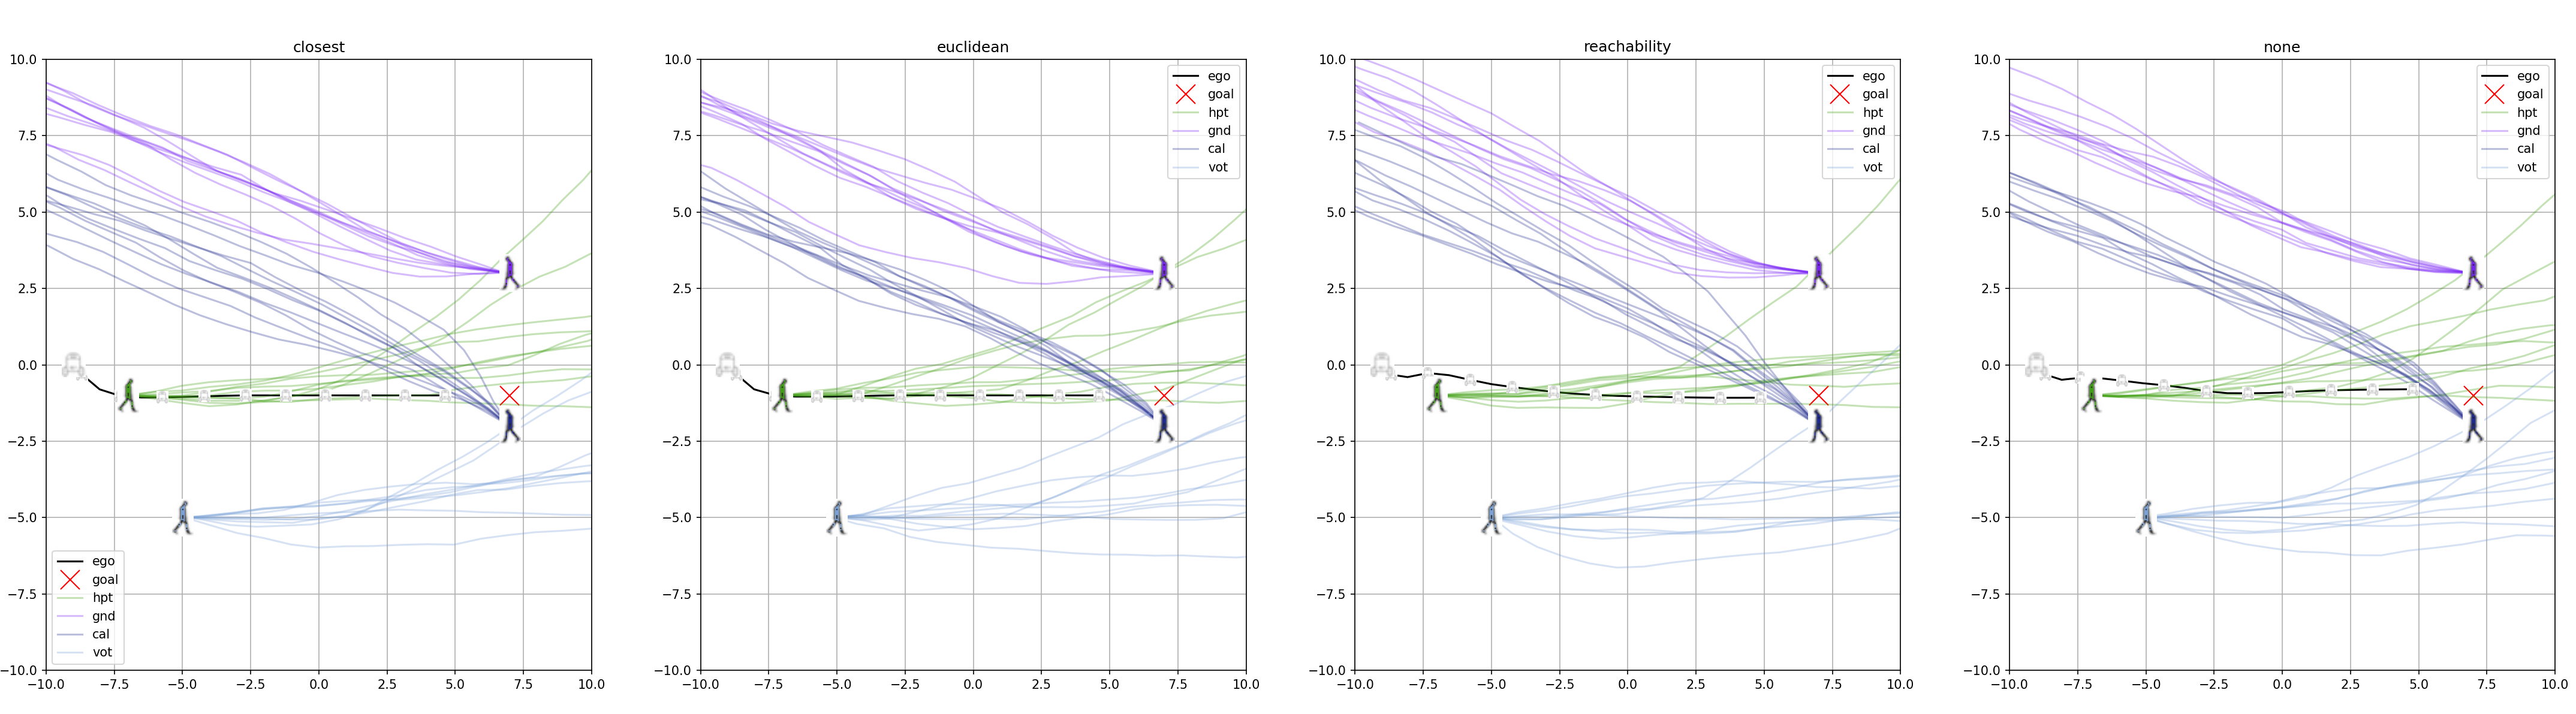
\includegraphics[width=\textwidth]{images/attention.png}
\end{center}
\caption{Trajectory Optimization with different attention modules. From left to right: euclidean, closest, reachability and without the use of attention. For further information please have a look at \href{https://github.com/simon-schaefer/mantrap/blob/master/examples/attention.ipynb}{attention notebook}.}
\label{img:attention}
\end{figure}
